\documentclass[a4paper]{article}

\usepackage{array}
\usepackage{listings}
\usepackage{appendix}
\usepackage{hyperref}
\usepackage{graphicx}
\usepackage{numprint}
\usepackage{booktabs}
\usepackage{subcaption}
\usepackage{listings}
\usepackage[T1]{fontenc}

\usepackage{hyperref}
\hypersetup{
  colorlinks=true,
  linkcolor=blue,
  filecolor=magenta,
  urlcolor=cyan,
}
\npdecimalsign{.}
\nprounddigits{4}

\title{S2-NRT Conistency Post Security Patch}
\date{25 August 2020}
\author{Josh Sixsmith and Imam Alam}

\begin{document}
  \pagenumbering{gobble}
  \maketitle
  \newpage
  \pagenumbering{arabic}

  \section{Introduction}

    \begin{flushleft}
      The prototype Sentinel-2 Near Real Time processing system deployed on Amazon Web Service has not been upgraded in at least 3 years, and has been flagged by Geoscience Australia IT services as a security concern. \par
      The whole NRT processing pipeline needs a major upgrade as the data produced from the system is inconsistent with the current definitive production system, which itself also needs a major upgrade in order to benefit from the updgrade ancillary sources. \par
      Whilst upgrading both the NRT and definitive deployments would be beneficial, the decision was made to only patch the machines on AWS and deploy the same ard-pipeline versions as a quicker turn around. \par
      The data outputs from DEA's NRT system are already known to be not correct; As such, the results from this report are not to evaluate the correctness, merely ensure that the results are consistent with the previous version.
    \end{flushleft}

    \subsection{Processing environments}
    \label{sec:environ}
      \begin{itemize}
        \item AWS
          \begin{itemize}
            \item wagl-5.0.5+33.g94f1105.dirty
            \item MODTRAN-5.2.1
          \end{itemize}
        \item AWS (patched machines)
          \begin{itemize}
            \item wagl-5.0.5+33.g94f1105.dirty
            \item MODTRAN-5.2.1
          \end{itemize}
      \end{itemize}

    \subsection{Base input data}

      ESA Sentinel-2 L1C (packaged by Sinergise)

    \subsection{Acquisition Period}

      2020/08/21

    \subsection{Reported Metrics}
      \begin{itemize}
        \item Minimum residual
        \item Maximum residual
        \item Percentage of pixels that are different
        \item Min and Max percentage of pixels that have changed categorical value
      \end{itemize}

    \subsection{Measurements}
      \begin{itemize}
        \item nbar\_coastal\_aerosol
        \item nbart\_coastal\_aerosol
        \item nbar\_blue
        \item nbart\_blue
        \item nbar\_green
        \item nbart\_green
        \item nbar\_red
        \item nbart\_red
        \item nbar\_red\_edge\_1
        \item nbart\_red\_edge\_1
        \item nbar\_red\_edge\_2
        \item nbart\_red\_edge\_2
        \item nbar\_red\_edge\_3
        \item nbart\_red\_edge\_3
        \item nbar\_nir\_1
        \item nbart\_nir\_1
        \item nbar\_nir\_2
        \item nbart\_nir\_2
        \item nbar\_swir\_2
        \item nbart\_swir\_2
        \item nbar\_swir\_3
        \item nbart\_swir\_3
        \item fmask
        \item terrain\_shadow
        \item nbar\_contiguity
        \item nbart\_contiguity
        \item solar\_azimuth
        \item solar\_zenith
        \item azimuthal\_exiting
        \item azimuthal\_incident
        \item exiting
        \item incident
      \end{itemize}

    \subsection{Other Assessments}
      \begin{itemize}
        \item GQA (Geometric Quality Assessment)
        \item Software Versions
        \item File Naming Consistency
        \item Quicklook Images
      \end{itemize}

    \section{Method}

      \begin{flushleft}
        10 Sentinel-2 L1C acquisitions from the 21st August 2020 were processed on both the old and new NRT AWS system deployments. The outputs from the new system were then compared and evaluated with those produced from the old system.
      \end{flushleft}

    \subsection{Rationale}

      \begin{flushleft}
        As the exact same versions of software was deployed for the new system, we expect there to be little or no difference when comparing the datasets. \par
        While extrema are reported (maximal and minimal residuals), they are often misinterpreted leading to biased assumptions as they don't describe the proportionality of change. The proportionality of change is what the aforementioned metrics are designed to describe. \par
        The percent different was simply describing the proportionality of change. For routine integration tests, it is ideal to have this number closer 0. As routine testing that is occurring on the same machine should exhibit less noise in floating point calculations. If deploying the codebase to a different machine, it is expected that there will be some floating point differences. This can occur due to slight differences in machine architecture, and/or different compilers. As such, this metric coupled with minimal and maximal differences/residuals, can help in aiding a user to ignore noise such as compiler or machine architecture differences. \par
        Changes in ancillary data used as input into the processing pipeline can result in minor differences, and should be taken into consideration when undertaking the evaluation.
      \end{flushleft}

  \newpage

  \section{Results}

    \subsection{Continental overview}

    \begin{flushleft}
      The following tables are reporting on the extrema (min and max) of difference for the different processing environments. \par
      In other words the total minimum and maximum of change in percent reflectance for a given measurement across all acquisition samples. \par
    \end{flushleft}

    \begin{table}[ht!]
      \caption{Minimum difference in surface reflectance (units are \% reflectance)}\label{table:1}
      \centering
      \begin{tabular}{cc} \midrule
        \textbf{Measurement} & \textbf{Minimum} \\ \midrule
        nbar\_coastal\_aerosol & -0.02 \\
        nbart\_coastal\_aerosol & -0.02 \\
        nbar\_blue & -0.03 \\
        nbart\_blue & -0.03 \\
        nbar\_green & -0.06 \\
        nbart\_green & -0.06 \\
        nbar\_red & -0.21 \\
        nbart\_red & -0.21 \\
        nbar\_red\_edge\_1 & -1.06 \\
        nbart\_red\_edge\_1 & -1.06 \\
        nbar\_red\_edge\_2 & -0.9 \\
        nbart\_red\_edge\_2 & -0.9 \\
        nbar\_red\_edge\_3 & -0.15 \\
        nbart\_red\_edge\_3 & -0.15 \\
        nbar\_nir\_1 & -1.23 \\
        nbart\_nir\_1 & -1.23 \\
        nbar\_nir\_2 & -0.06 \\
        nbart\_nir\_2 & -0.06 \\
        nbar\_swir\_2 & -0.13 \\
        nbart\_swir\_2 & -0.13 \\
        nbar\_swir\_3 & -0.89 \\
        nbart\_swir\_3 & -0.91 \\ \midrule
      \end{tabular}
    \end{table}

    \begin{table}[ht!]
      \caption{Maximum difference in surface reflectance (units are \% reflectance)}\label{table:2}
      \centering
      \begin{tabular}{cc} \midrule
        \textbf{Measurement} & \textbf{Maximum} \\ \midrule
        nbar\_coastal\_aerosol & 0.01 \\
        nbart\_coastal\_aerosol & 0.01 \\
        nbar\_blue & 0.01 \\
        nbart\_blue & 0.01 \\
        nbar\_green & 0.01 \\
        nbart\_green & 0.01 \\
        nbar\_red & 0.01 \\
        nbart\_red & 0.01 \\
        nbar\_red\_edge\_1 & 0.05 \\
        nbart\_red\_edge\_1 & 0.05 \\
        nbar\_red\_edge\_2 & 0.04 \\
        nbart\_red\_edge\_2 & 0.04 \\
        nbar\_red\_edge\_3 & 0.01 \\
        nbart\_red\_edge\_3 & 0.01 \\
        nbar\_nir\_1 & 0.05 \\
        nbart\_nir\_1 & 0.05 \\
        nbar\_nir\_2 & 0.01 \\
        nbart\_nir\_2 & 0.01 \\
        nbar\_swir\_2 & 0.01 \\
        nbart\_swir\_2 & 0.01 \\
        nbar\_swir\_3 & 0.04 \\
        nbart\_swir\_3 & 0.04 \\ \midrule
      \end{tabular}
    \end{table}

  \newpage

    \begin{table}[ht!]
      \caption{Maximum difference for the angular measurements (units are degrees)}\label{table:3}
      \centering
      \begin{tabular}{cc} \midrule
        \textbf{Measurement} & \textbf{Maximum} \\ \midrule
        solar\_azimuth & 0.0 \\
        solar\_zenith & 0.0 \\
        satellite\_azimuth & 0.0 \\
        satellite\_view & 0.0 \\
        azimuthal\_exiting & 0.0 \\
        azimuthal\_incident & 0.0 \\
        exiting & 0.0 \\
        incident & 0.0 \\ \midrule
      \end{tabular}
    \end{table}

  \clearpage

    \begin{flushleft}
      Table~\ref{table:4}, below, represents the proportion of pixels that a different (excluding those pixels that may have changed to a \textit{Null} or vice versa). The maximum percent of difference for each measurement is derived from all 10 acquisition samples.
    \end{flushleft}

    \begin{table}[ht!]
      \caption{Percentage of pixels (acquisition wide) that are different}\label{table:4}
      \centering
      \begin{tabular}{cc} \midrule
        \textbf{Measurement} & \textbf{Percentage} \\ \midrule
        nbar\_coastal\_aerosol & 25.805825921120316 \\
        nbart\_coastal\_aerosol & 25.83178824382657 \\
        nbar\_blue & 47.5397119960226 \\
        nbart\_blue & 47.59214201039111 \\
        nbar\_green & 87.566195865309 \\
        nbart\_green & 87.58792387831842 \\
        nbar\_red & 99.98822664821948 \\
        nbart\_red & 99.98834774886063 \\
        nbar\_red\_edge\_1 & 100.0 \\
        nbart\_red\_edge\_1 & 100.0 \\
        nbar\_red\_edge\_2 & 100.0 \\
        nbart\_red\_edge\_2 & 100.0 \\
        nbar\_red\_edge\_3 & 99.99998341080487 \\
        nbart\_red\_edge\_3 & 99.9999867286439 \\
        nbar\_nir\_1 & 100.0 \\
        nbart\_nir\_1 & 100.0 \\
        nbar\_nir\_2 & 99.9447812051055 \\
        nbart\_nir\_2 & 99.94410436594437 \\
        nbar\_swir\_2 & 99.9893397832124 \\
        nbart\_swir\_2 & 99.98920043397335 \\
        nbar\_swir\_3 & 100.0 \\
        nbart\_swir\_3 & 100.0 \\
        solar\_azimuth & 0.0 \\
        solar\_zenith & 0.0 \\
        satellite\_azimuth & 0.0 \\
        satellite\_view & 0.0 \\
        azimuthal\_exiting & 0.0 \\
        azimuthal\_incident & 0.0 \\
        exiting\_angle & 0.0 \\
        incident\_angle & 0.0 \\ \midrule
      \end{tabular}
    \end{table}

      \begin{flushleft}
        The minimum and maximum difference are mostly reporting less than 1\% change in surface reflectance. \par
        Overall, it appears that there is more of a negative change in surface reflectance, with 10 of the dataset measurements reporting a negative 1\% change in surface reflectance. \par
        This might have an affect on some aquatic based remote sensing applications. \par
        The proportionality of differences is quite high, with some measurements recording 100\% of pixels changing. Further investigation is required as it simply could be due to slight differences in floating point calculations, as well as slight differences in input ancillary. \par
        The angular measurements are all reporting no change. This suggests that differences in floating point calculations is less likely, and the high proportionality of change in the reflectance measurements is most likely due to differences in ancillary input.
      \end{flushleft}


      \begin{flushleft}
        Table~\ref{table:5} and Table~\ref{table:6}, below, represents the minimum and maximum percentage of pixels in a given category within the Fmask schema changing to another category. i.e. Pixels originally classified as Clear and now being classified as Cloud. \par
        A value of 100 represents 100\%, and indicates that all pixels from all granules mapped entirely to the corresponding category. A NaN implies no recorded pixels for that category. \par
        A good indicator for data consistency for a category mapping to the same category, say cloud to cloud, is a value close to 100\%. For a category mapping to a different category, say cloud to snow, a value close to 0\% or NaN, is also good indicator for data consistency.
      \end{flushleft}

  \clearpage

    \begin{table}[ht!]
      \caption{Minimum percentage of categorical change within Fmask}\label{table:5}
      \centering
      \begin{tabular}{ccccccc} \midrule
        & \textbf{Null} & \textbf{Clear} & \textbf{Cloud} & \textbf{Cloud Shadow} & \textbf{Snow} & \textbf{Water} \\ \midrule
        \textbf{Null} & 100 & NaN & NaN & NaN & NaN & NaN \\
        \textbf{Clear} & NaN & 100 & NaN & NaN & NaN & NaN \\
        \textbf{Cloud} & NaN & NaN & 100 & NaN & NaN & NaN \\
        \textbf{Cloud Shadow} & NaN & NaN & NaN & 100 & NaN & NaN \\
        \textbf{Snow} & NaN & NaN & NaN & NaN & 100 & NaN \\
        \textbf{Water} & NaN & NaN & NaN & NaN & NaN & 100 \\
      \end{tabular}
    \end{table}

    \begin{table}[ht!]
      \caption{Maximum percentage of categorical change within Fmask}\label{table:6}
      \centering
      \begin{tabular}{ccccccc} \midrule
        & \textbf{Null} & \textbf{Clear} & \textbf{Cloud} & \textbf{Cloud Shadow} & \textbf{Snow} & \textbf{Water} \\ \midrule
        \textbf{Null} & 100 & NaN & NaN & NaN & NaN & NaN \\
        \textbf{Clear} & NaN & 100 & NaN & NaN & NaN & NaN \\
        \textbf{Cloud} & NaN & NaN & 100 & NaN & NaN & NaN \\
        \textbf{Cloud Shadow} & NaN & NaN & NaN & 100 & NaN & NaN \\
        \textbf{Snow} & NaN & NaN & NaN & NaN & 100 & NaN \\
        \textbf{Water} & NaN & NaN & NaN & NaN & NaN & 100 \\
      \end{tabular}
    \end{table}

      \begin{flushleft}
        As you can see, for the 10 acquisitions, there is not a single pixel that has changed categorical states between the different processing environments.
      \end{flushleft}

  % \newpage

    \begin{flushleft}
      Table~\ref{table:7} and Table~\ref{table:8}, below, represents the minimum and maximum percentage of pixels, that are either contiguous or non-contiguous, changing from one category to another (or itself) \textit{nbart\_contiguity} measurement.
    \end{flushleft}

    \begin{table}[ht!]
      \caption{Minimum percentage of categorical change within the \textit{nbart\_contiguity} measurement}\label{table:7}
      \centering
      \begin{tabular}{ccc} \midrule
        & \textbf{Contiguous} & \textbf{Non-Contiguous} \\ \midrule
        \textbf{Contiguous} & 100.0 & NaN \\
        \textbf{Non-Contiguous} & NaN & 100 \\
      \end{tabular}
    \end{table}

    \begin{table}[ht!]
      \caption{Maximum percentage of categorical change within the \textit{nbart\_contiguity} measurement}\label{table:8}
      \centering
      \begin{tabular}{ccc} \midrule
        & \textbf{Contiguous} & \textbf{Non-Contiguous} \\ \midrule
        \textbf{Contiguous} & 100.0 & NaN \\
        \textbf{Non-Contiguous} & 0.22274195344693173 & 100.0 \\
      \end{tabular}
    \end{table}

    \begin{flushleft}
      For the \textit{nbart\_contiguity} measurements, there is a very minor (small number of pixels) that have changed categorical state. \par
      Investigating further into this issue, revealed that only 1 of the 10 acquisitions had this change of state. The locations for the change of state occurs along the edges of objects flagged as terrain shadow. \par
      As the number of pixels is very small, and at individual locations along object edges, we don't consider this to be a significant change, and unlikely to severely impact any application derived from this data.
    \end{flushleft}

    \begin{flushleft}
      Table~\ref{table:9} and Table~\ref{table:10}, below, represents the minimum and maximum percentage of pixels, that are either contiguous or non-contiguous, changing from one category to another (or itself) for the \textit{nbar\_contiguity} measurement.
    \end{flushleft}

    \begin{table}[ht!]
      \caption{Minimum percentage of categorical change within the \textit{oa\_nbar\_contiguity} measurement}\label{table:9}
      \centering
      \begin{tabular}{ccc} \midrule
        & \textbf{Contiguous} & \textbf{Non-Contiguous} \\ \midrule
        \textbf{Contiguous} & 100 & NaN \\
        \textbf{Non-Contiguous} & NaN & 100 \\
      \end{tabular}
    \end{table}

    \begin{table}[ht!]
      \caption{Maximum percentage of categorical change within the \textit{oa\_nbar\_contiguity} measurement}\label{table:10}
      \centering
      \begin{tabular}{ccc} \midrule
        & \textbf{Contiguous} & \textbf{Non-Contiguous} \\ \midrule
        \textbf{Contiguous} & 100.0 & NaN \\
        \textbf{Non-Contiguous} & NaN & 100.0 \\
      \end{tabular}
    \end{table}

    \begin{flushleft}
      For the \textit{nbar\_contiguity} measurement, there is no categorical change for pixels between the two different processing environments.
    \end{flushleft}

  % \vspace{5mm}
  \clearpage

    \begin{flushleft}
      Table~\ref{table:11} and Table~\ref{table:12}, below, represents the minimum and maximum percentage of pixels, that are either shadow or non-shadow, changing from one category to another (or itself) for the \textit{terrain\_shadow} measurement.
    \end{flushleft}

    \begin{table}[ht!]
      \caption{Minimum percentage of categorical change within the \textit{oa\_combined\_terrain\_shadow} measurement}\label{table:11}
      \centering
      \begin{tabular}{ccc} \midrule
        & \textbf{Shadow} & \textbf{Not-Shadow} \\ \midrule
        \textbf{Shadow} & 100.0 & NaN \\
        \textbf{Not-Shadow} & NaN & 100.0 \\
      \end{tabular}
    \end{table}

    \begin{table}[ht!]
      \caption{Maximum percentage of categorical change within the \textit{oa\_combined\_terrain\_shadow} measurement}\label{table:12}
      \centering
      \begin{tabular}{ccc} \midrule
        & \textbf{Shadow} & \textbf{Not-Shadow} \\ \midrule
        \textbf{Shadow} & 100.0 & 2.941176470588235 \\
        \textbf{Not-Shadow} & NaN & 100.0 \\
      \end{tabular}
    \end{table}

    \begin{flushleft}
      For the \textit{terrain\_shadow} measurement, there is a small change in categorical state. Further investigation identified only 2 of the 10 acquisitions had a change of state (shaded to unshaded). \par
      Whilst the proportion of change appears quite high, it is only relative to the total number of pixels for that category, in this case shadow, not for the total number of pixels in the image. The acquisition with the highest proportion of change only had 68 pixels detected as shadow, meaning that only 2 pixels changed state. \par
      As such, we don't consider this to be significant, nor have any significant impact on a derived application.
    \end{flushleft}

    \subsection{Spatial Distribution}

      \begin{flushleft}
        The following section presents the impact of change spatially across the 10 sample acquisitions. \par
        The idea is to pictorially represent whether there are any spatial patterns or associations with the changes in processing environments. \par
        This has an added advantage of informing users that while there might be change within the data collection that is being processed, their application may not be affected if differences are located in particular regions.
      \end{flushleft}

  \clearpage

    \subsubsection{Extrema Differences (\textit{min, max})}

      \begin{flushleft}
        The section is to present the spatial distribution of the residuals, and in particular, highlight the locations of extrema, and any spatial patterns that may be visible across the 10 sample acquisitions. \par
      \end{flushleft}

      \begin{figure}[h!]
        \centering
          \begin{subfigure}[l]{.4\linewidth}
            \hspace{-32mm}
            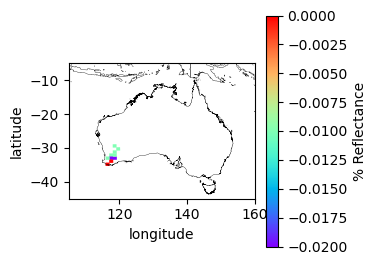
\includegraphics[scale=0.9]{plots/nbart/nbart_coastal_aerosol-MinResidual.png}
            \caption{Minimum residual}
          \end{subfigure}
%
          \begin{subfigure}[r]{.4\linewidth}
            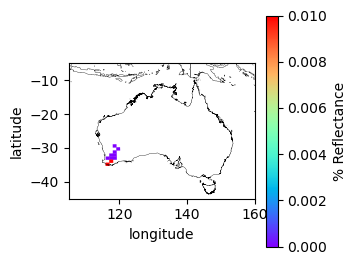
\includegraphics[scale=0.9]{plots/nbart/nbart_coastal_aerosol-MaxResidual.png}
            \caption{Maximum residual}
          \end{subfigure}
        \caption{NBART;\@ Coastal Aerosol Band}\label{figure:1}
      \end{figure}

      \begin{figure}[h!]
        \centering
          \begin{subfigure}[l]{.4\linewidth}
            \hspace{-32mm}
            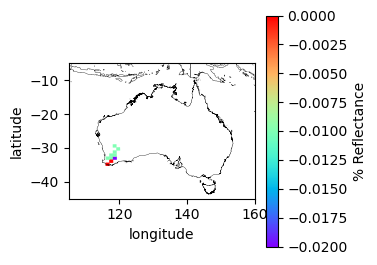
\includegraphics[scale=0.9]{plots/nbar/nbar_coastal_aerosol-MinResidual.png}
            \caption{Minimum residual}
          \end{subfigure}
%
          \begin{subfigure}[r]{.4\linewidth}
            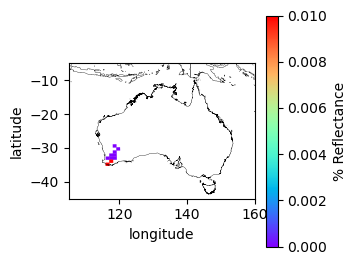
\includegraphics[scale=0.9]{plots/nbar/nbar_coastal_aerosol-MaxResidual.png}
            \caption{Maximum residual}
          \end{subfigure}
        \caption{NBAR;\@ Coastal Aerosol Band}\label{figure:2}
      \end{figure}

  \clearpage

      \begin{figure}[h!]
        \centering
          \begin{subfigure}[l]{.4\linewidth}
            \hspace{-32mm}
            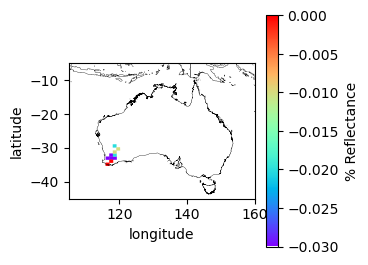
\includegraphics[scale=0.9]{plots/nbart/nbart_blue-MinResidual.png}
            \caption{Minimum residual}
          \end{subfigure}
%
          \begin{subfigure}[r]{.4\linewidth}
            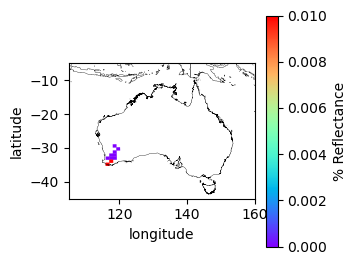
\includegraphics[scale=0.9]{plots/nbart/nbart_blue-MaxResidual.png}
            \caption{Maximum residual}
          \end{subfigure}
        \caption{NBART;\@ Blue Band}\label{figure:3}
      \end{figure}

      \begin{figure}[h!]
        \centering
          \begin{subfigure}[l]{.4\linewidth}
            \hspace{-32mm}
            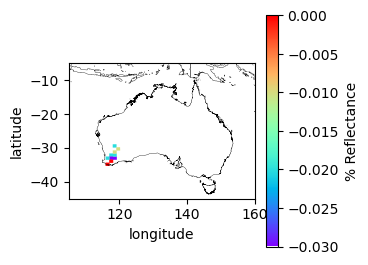
\includegraphics[scale=0.9]{plots/nbar/nbar_blue-MinResidual.png}
            \caption{Minimum residual}
          \end{subfigure}
%
          \begin{subfigure}[r]{.4\linewidth}
            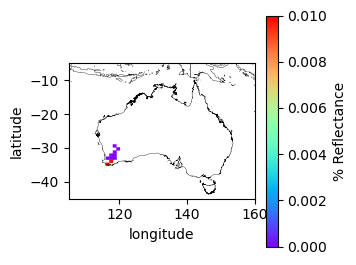
\includegraphics[scale=0.9]{plots/nbar/nbar_blue-MaxResidual.png}
            \caption{Maximum residual}
          \end{subfigure}
        \caption{NBAR;\@ Blue Band}\label{figure:4}
      \end{figure}

  \clearpage

      \begin{figure}[h!]
        \centering
          \begin{subfigure}[l]{.4\linewidth}
            \hspace{-32mm}
            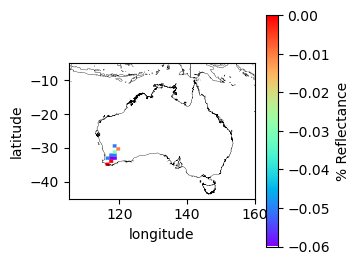
\includegraphics[scale=0.9]{plots/nbart/nbart_green-MinResidual.png}
            \caption{Minimum residual}
          \end{subfigure}
%
          \begin{subfigure}[r]{.4\linewidth}
            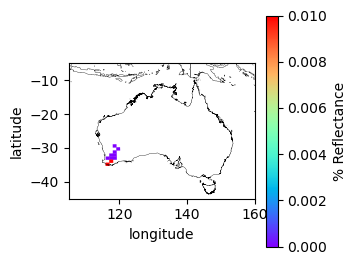
\includegraphics[scale=0.9]{plots/nbart/nbart_green-MaxResidual.png}
            \caption{Maximum residual}
          \end{subfigure}
        \caption{NBART;\@ Green Band}\label{figure:5}
      \end{figure}

      \begin{figure}[h!]
        \centering
          \begin{subfigure}[l]{.4\linewidth}
            \hspace{-32mm}
            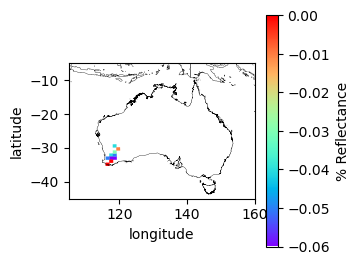
\includegraphics[scale=0.9]{plots/nbar/nbar_green-MinResidual.png}
            \caption{Minimum residual}
          \end{subfigure}
%
          \begin{subfigure}[r]{.4\linewidth}
            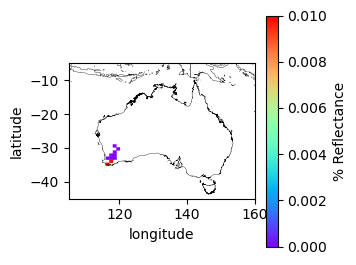
\includegraphics[scale=0.9]{plots/nbar/nbar_green-MaxResidual.png}
            \caption{Maximum residual}
          \end{subfigure}
        \caption{NBAR;\@ Green Band}\label{figure:6}
      \end{figure}

  \clearpage

      \begin{figure}[h!]
        \centering
          \begin{subfigure}[l]{.4\linewidth}
            \hspace{-32mm}
            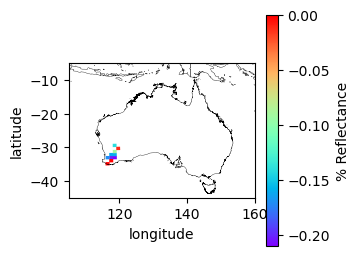
\includegraphics[scale=0.9]{plots/nbart/nbart_red-MinResidual.png}
            \caption{Minimum residual}
          \end{subfigure}
%
          \begin{subfigure}[r]{.4\linewidth}
            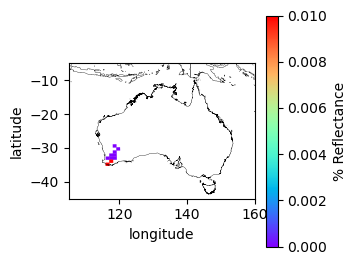
\includegraphics[scale=0.9]{plots/nbart/nbart_red-MaxResidual.png}
            \caption{Maximum residual}
          \end{subfigure}
        \caption{NBART;\@ Red Band}\label{figure:7}
      \end{figure}

      \begin{figure}[h!]
        \centering
          \begin{subfigure}[l]{.4\linewidth}
            \hspace{-32mm}
            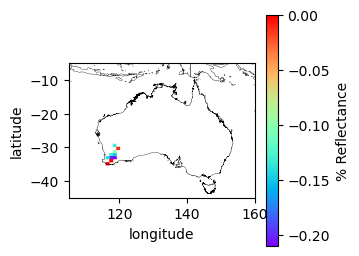
\includegraphics[scale=0.9]{plots/nbar/nbar_red-MinResidual.png}
            \caption{Minimum residual}
          \end{subfigure}
%
          \begin{subfigure}[r]{.4\linewidth}
            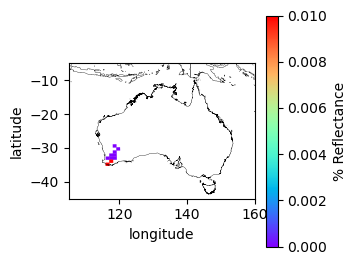
\includegraphics[scale=0.9]{plots/nbar/nbar_red-MaxResidual.png}
            \caption{Maximum residual}
          \end{subfigure}
        \caption{NBAR;\@ Red Band}\label{figure:8}
      \end{figure}

  \clearpage

      \begin{figure}[h!]
        \centering
          \begin{subfigure}[l]{.4\linewidth}
            \hspace{-32mm}
            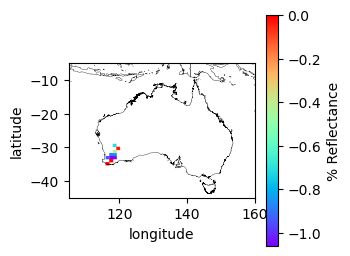
\includegraphics[scale=0.9]{plots/nbart/nbart_red_edge_1-MinResidual.png}
            \caption{Minimum residual}
          \end{subfigure}
%
          \begin{subfigure}[r]{.4\linewidth}
            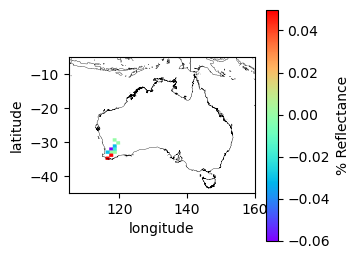
\includegraphics[scale=0.9]{plots/nbart/nbart_red_edge_1-MaxResidual.png}
            \caption{Maximum residual}
          \end{subfigure}
        \caption{NBART;\@ Red Edge 1 Band}\label{figure:9}
      \end{figure}

      \begin{figure}[h!]
        \centering
          \begin{subfigure}[l]{.4\linewidth}
            \hspace{-32mm}
            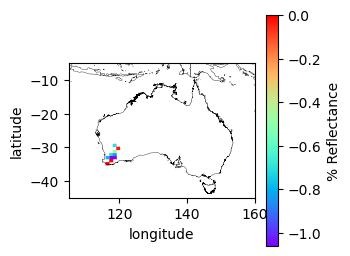
\includegraphics[scale=0.9]{plots/nbar/nbar_red_edge_1-MinResidual.png}
            \caption{Minimum residual}
          \end{subfigure}
%
          \begin{subfigure}[r]{.4\linewidth}
            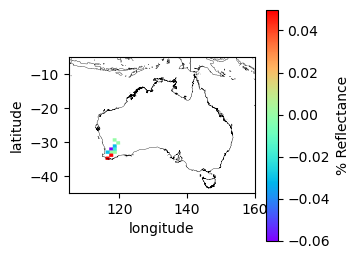
\includegraphics[scale=0.9]{plots/nbar/nbar_red_edge_1-MaxResidual.png}
            \caption{Maximum residual}
          \end{subfigure}
        \caption{NBAR;\@ Red Edge 1 Band}\label{figure:10}
      \end{figure}

  \clearpage

      \begin{figure}[h!]
        \centering
          \begin{subfigure}[l]{.4\linewidth}
            \hspace{-32mm}
            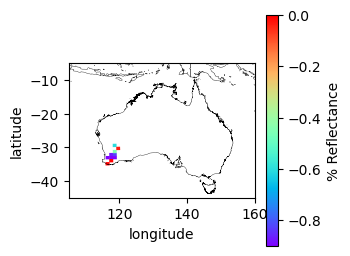
\includegraphics[scale=0.9]{plots/nbart/nbart_red_edge_2-MinResidual.png}
            \caption{Minimum residual}
          \end{subfigure}
%
          \begin{subfigure}[r]{.4\linewidth}
            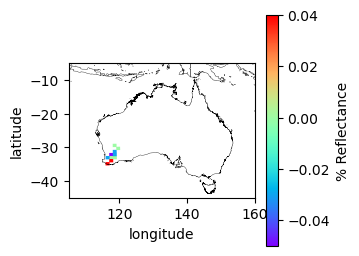
\includegraphics[scale=0.9]{plots/nbart/nbart_red_edge_2-MaxResidual.png}
            \caption{Maximum residual}
          \end{subfigure}
        \caption{NBART;\@ Red Edge 2 Band}\label{figure:11}
      \end{figure}

      \begin{figure}[h!]
        \centering
          \begin{subfigure}[l]{.4\linewidth}
            \hspace{-32mm}
            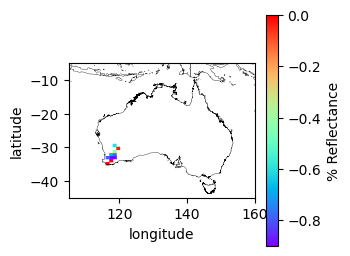
\includegraphics[scale=0.9]{plots/nbar/nbar_red_edge_2-MinResidual.png}
            \caption{Minimum residual}
          \end{subfigure}
%
          \begin{subfigure}[r]{.4\linewidth}
            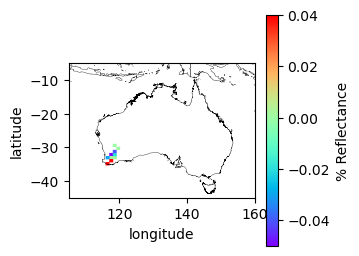
\includegraphics[scale=0.9]{plots/nbar/nbar_red_edge_2-MaxResidual.png}
            \caption{Maximum residual}
          \end{subfigure}
        \caption{NBAR;\@ Red Edge 2 Band}\label{figure:12}
      \end{figure}

  \clearpage

      \begin{figure}[h!]
        \centering
          \begin{subfigure}[l]{.4\linewidth}
            \hspace{-32mm}
            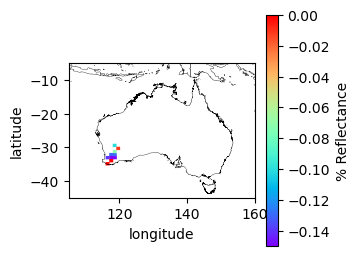
\includegraphics[scale=0.9]{plots/nbart/nbart_red_edge_3-MinResidual.png}
            \caption{Minimum residual}
          \end{subfigure}
%
          \begin{subfigure}[r]{.4\linewidth}
            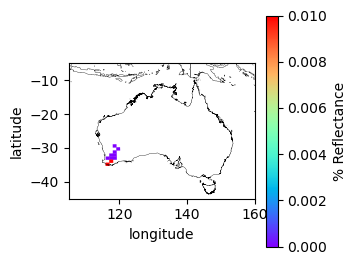
\includegraphics[scale=0.9]{plots/nbart/nbart_red_edge_3-MaxResidual.png}
            \caption{Maximum residual}
          \end{subfigure}
        \caption{NBART;\@ Red Edge 3 Band}\label{figure:13}
      \end{figure}

      \begin{figure}[h!]
        \centering
          \begin{subfigure}[l]{.4\linewidth}
            \hspace{-32mm}
            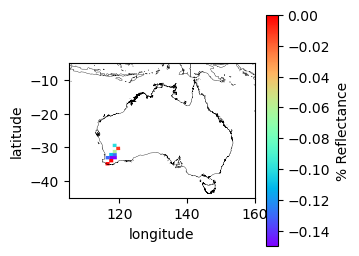
\includegraphics[scale=0.9]{plots/nbar/nbar_red_edge_3-MinResidual.png}
            \caption{Minimum residual}
          \end{subfigure}
%
          \begin{subfigure}[r]{.4\linewidth}
            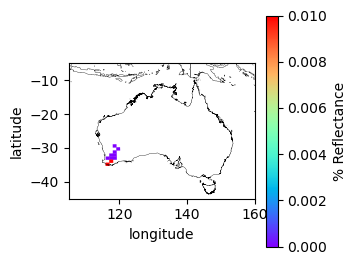
\includegraphics[scale=0.9]{plots/nbar/nbar_red_edge_3-MaxResidual.png}
            \caption{Maximum residual}
          \end{subfigure}
        \caption{NBAR;\@ Red Edge 3 Band}\label{figure:14}
      \end{figure}

  \clearpage

      \begin{figure}[h!]
        \centering
          \begin{subfigure}[l]{.4\linewidth}
            \hspace{-32mm}
            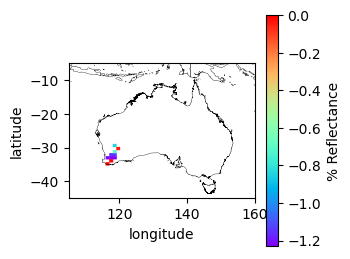
\includegraphics[scale=0.9]{plots/nbart/nbart_nir_1-MinResidual.png}
            \caption{Minimum residual}
          \end{subfigure}
%
          \begin{subfigure}[r]{.4\linewidth}
            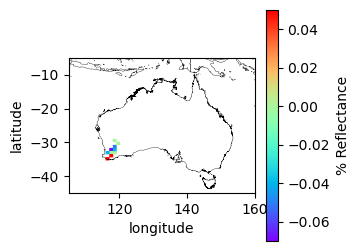
\includegraphics[scale=0.9]{plots/nbart/nbart_nir_1-MaxResidual.png}
            \caption{Maximum residual}
          \end{subfigure}
        \caption{NBART;\@ NIR-1 Band}\label{figure:15}
      \end{figure}

      \begin{figure}[h!]
        \centering
          \begin{subfigure}[l]{.4\linewidth}
            \hspace{-32mm}
            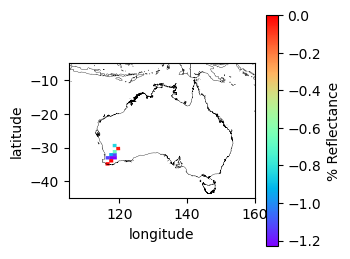
\includegraphics[scale=0.9]{plots/nbar/nbar_nir_1-MinResidual.png}
            \caption{Minimum residual}
          \end{subfigure}
%
          \begin{subfigure}[r]{.4\linewidth}
            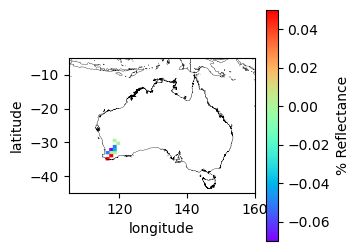
\includegraphics[scale=0.9]{plots/nbar/nbar_nir_1-MaxResidual.png}
            \caption{Maximum residual}
          \end{subfigure}
        \caption{NBAR;\@ NIR-1 Band}\label{figure:16}
      \end{figure}

  \clearpage

      \begin{figure}[h!]
        \centering
          \begin{subfigure}[l]{.4\linewidth}
            \hspace{-32mm}
            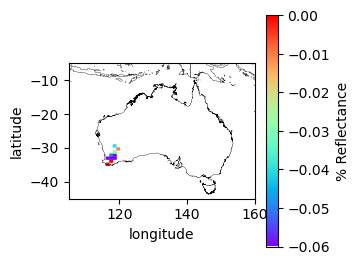
\includegraphics[scale=0.9]{plots/nbart/nbart_nir_2-MinResidual.png}
            \caption{Minimum residual}
          \end{subfigure}
%
          \begin{subfigure}[r]{.4\linewidth}
            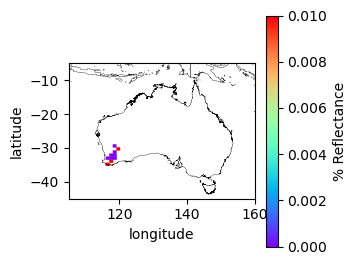
\includegraphics[scale=0.9]{plots/nbart/nbart_nir_2-MaxResidual.png}
            \caption{Maximum residual}
          \end{subfigure}
        \caption{NBART;\@ NIR-2 Band}\label{figure:17}
      \end{figure}

      \begin{figure}[h!]
        \centering
          \begin{subfigure}[l]{.4\linewidth}
            \hspace{-32mm}
            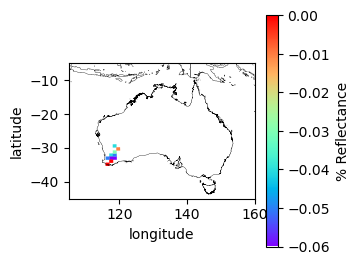
\includegraphics[scale=0.9]{plots/nbar/nbar_nir_2-MinResidual.png}
            \caption{Minimum residual}
          \end{subfigure}
%
          \begin{subfigure}[r]{.4\linewidth}
            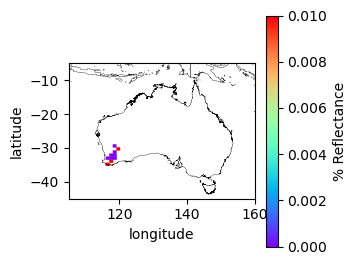
\includegraphics[scale=0.9]{plots/nbar/nbar_nir_2-MaxResidual.png}
            \caption{Maximum residual}
          \end{subfigure}
        \caption{NBAR;\@ NIR-2 Band}\label{figure:18}
      \end{figure}

  \clearpage

      \begin{figure}[h!]
        \centering
          \begin{subfigure}[l]{.4\linewidth}
            \hspace{-32mm}
            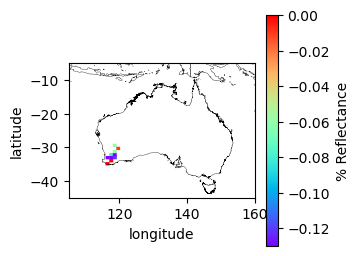
\includegraphics[scale=0.9]{plots/nbart/nbart_swir_2-MinResidual.png}
            \caption{Minimum residual}
          \end{subfigure}
%
          \begin{subfigure}[r]{.4\linewidth}
            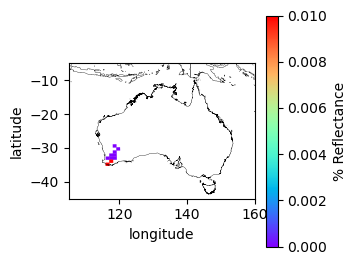
\includegraphics[scale=0.9]{plots/nbart/nbart_swir_2-MaxResidual.png}
            \caption{Maximum residual}
          \end{subfigure}
        \caption{NBART;\@ SWIR-2 Band}\label{figure:19}
      \end{figure}

      \begin{figure}[h!]
        \centering
          \begin{subfigure}[l]{.4\linewidth}
            \hspace{-32mm}
            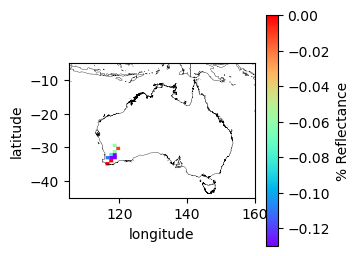
\includegraphics[scale=0.9]{plots/nbar/nbar_swir_2-MinResidual.png}
            \caption{Minimum residual}
          \end{subfigure}
%
          \begin{subfigure}[r]{.4\linewidth}
            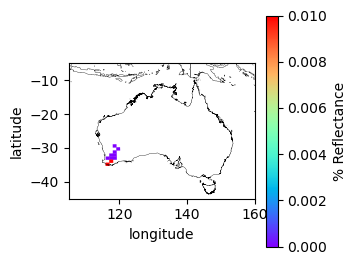
\includegraphics[scale=0.9]{plots/nbar/nbar_swir_2-MaxResidual.png}
            \caption{Maximum residual}
          \end{subfigure}
        \caption{NBAR;\@ SWIR-2 Band}\label{figure:20}
      \end{figure}

  \clearpage

      \begin{figure}[h!]
        \centering
          \begin{subfigure}[l]{.4\linewidth}
            \hspace{-32mm}
            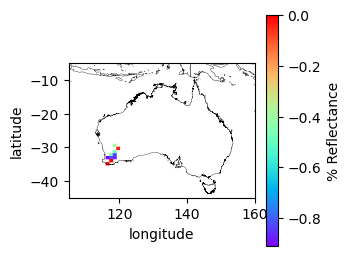
\includegraphics[scale=0.9]{plots/nbart/nbart_swir_3-MinResidual.png}
            \caption{Minimum residual}
          \end{subfigure}
%
          \begin{subfigure}[r]{.4\linewidth}
            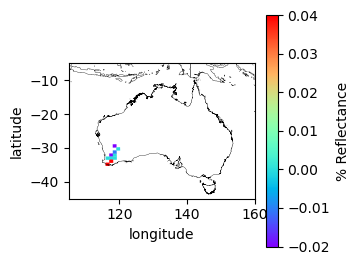
\includegraphics[scale=0.9]{plots/nbart/nbart_swir_3-MaxResidual.png}
            \caption{Maximum residual}
          \end{subfigure}
        \caption{NBART;\@ SWIR-3 Band}\label{figure:21}
      \end{figure}

      \begin{figure}[h!]
        \centering
          \begin{subfigure}[l]{.4\linewidth}
            \hspace{-32mm}
            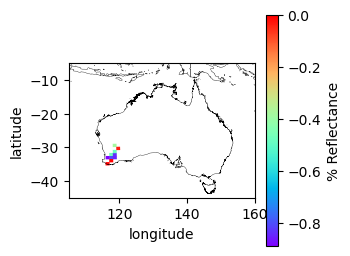
\includegraphics[scale=0.9]{plots/nbar/nbar_swir_3-MinResidual.png}
            \caption{Minimum residual}
          \end{subfigure}
%
          \begin{subfigure}[r]{.4\linewidth}
            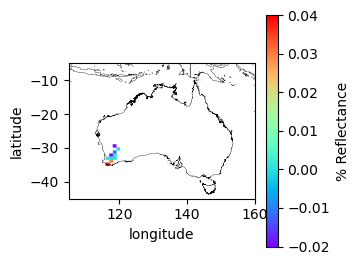
\includegraphics[scale=0.9]{plots/nbar/nbar_swir_3-MaxResidual.png}
            \caption{Maximum residual}
          \end{subfigure}
        \caption{NBAR;\@ SWIR-3 Band}\label{figure:22}
      \end{figure}

  \clearpage

    \subsubsection{Proportion of Differences (\textit{\% of pixels != 0})}

      \begin{flushleft}
        The section is to inform the spatial distribution of the proportionality of pixels that are different, i.e. the residual is != 0. \par
        Two key pieces of information can be inferred here:
        \begin{enumerate}
          \item The extremities for the proportion of non-zero residuals
          \item A spatial representation of non-zero residuals
        \end{enumerate}
      \end{flushleft}

      \begin{figure}[h!]
        \centering
          \begin{subfigure}[l]{.4\linewidth}
            \hspace{-32mm}
            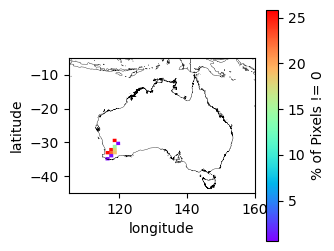
\includegraphics[scale=0.9]{plots/nbart/nbart_coastal_aerosol-PercentDifferent.png}
            \caption{NBART}
          \end{subfigure}
%
          \begin{subfigure}[r]{.4\linewidth}
            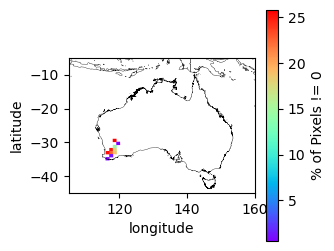
\includegraphics[scale=0.9]{plots/nbar/nbar_coastal_aerosol-PercentDifferent.png}
            \caption{NBAR}
          \end{subfigure}
        \caption{Coastal Aerosol Band \% Pixels != 0}\label{figure:23}
      \end{figure}

      \begin{figure}[h!]
        \centering
          \begin{subfigure}[l]{.4\linewidth}
            \hspace{-32mm}
            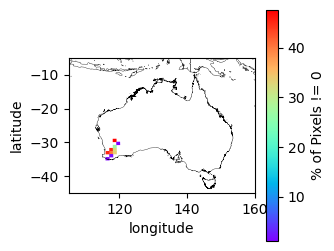
\includegraphics[scale=0.9]{plots/nbart/nbart_blue-PercentDifferent.png}
            \caption{NBART}
          \end{subfigure}
%
          \begin{subfigure}[r]{.4\linewidth}
            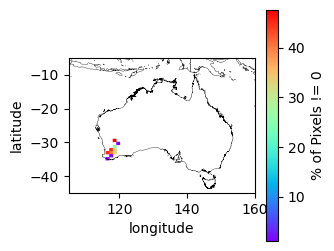
\includegraphics[scale=0.9]{plots/nbar/nbar_blue-PercentDifferent.png}
            \caption{NBAR}
          \end{subfigure}
        \caption{Blue Band \% Pixels != 0}\label{figure:24}
      \end{figure}

  \clearpage

      \begin{figure}[h!]
        \centering
          \begin{subfigure}[l]{.4\linewidth}
            \hspace{-32mm}
            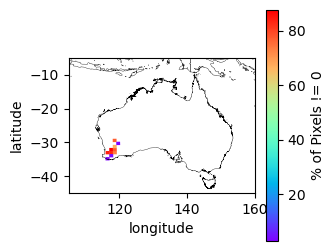
\includegraphics[scale=0.9]{plots/nbart/nbart_green-PercentDifferent.png}
            \caption{NBART}
          \end{subfigure}
%
          \begin{subfigure}[r]{.4\linewidth}
            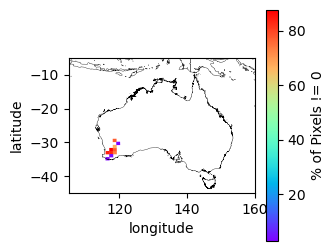
\includegraphics[scale=0.9]{plots/nbar/nbar_green-PercentDifferent.png}
            \caption{NBAR}
          \end{subfigure}
        \caption{Green Band \% Pixels != 0}\label{figure:25}
      \end{figure}

      \begin{figure}[h!]
        \centering
          \begin{subfigure}[l]{.4\linewidth}
            \hspace{-32mm}
            \includegraphics[scale=0.9]{plots/nbart/nbart_red-PercentDifferent.png}
            \caption{NBART}
          \end{subfigure}
%
          \begin{subfigure}[r]{.4\linewidth}
            \includegraphics[scale=0.9]{plots/nbar/nbar_red-PercentDifferent.png}
            \caption{NBAR}
          \end{subfigure}
        \caption{Red Band \% Pixels != 0}\label{figure:26}
      \end{figure}

  \clearpage

      \begin{figure}[h!]
        \centering
          \begin{subfigure}[l]{.4\linewidth}
            \hspace{-32mm}
            \includegraphics[scale=0.9]{plots/nbart/nbart_red_edge_1-PercentDifferent.png}
            \caption{NBART}
          \end{subfigure}
%
          \begin{subfigure}[r]{.4\linewidth}
            \includegraphics[scale=0.9]{plots/nbar/nbar_red_edge_1-PercentDifferent.png}
            \caption{NBAR}
          \end{subfigure}
        \caption{Red Edge 1 Band \% Pixels != 0}\label{figure:27}
      \end{figure}

      \begin{figure}[h!]
        \centering
          \begin{subfigure}[l]{.4\linewidth}
            \hspace{-32mm}
            \includegraphics[scale=0.9]{plots/nbart/nbart_red_edge_2-PercentDifferent.png}
            \caption{NBART}
          \end{subfigure}
%
          \begin{subfigure}[r]{.4\linewidth}
            \includegraphics[scale=0.9]{plots/nbar/nbar_red_edge_2-PercentDifferent.png}
            \caption{NBAR}
          \end{subfigure}
        \caption{Red Edge 2 Band \% Pixels != 0}\label{figure:28}
      \end{figure}

  \clearpage

      \begin{figure}[h!]
        \centering
          \begin{subfigure}[l]{.4\linewidth}
            \hspace{-32mm}
            \includegraphics[scale=0.9]{plots/nbart/nbart_red_edge_3-PercentDifferent.png}
            \caption{NBART}
          \end{subfigure}
%
          \begin{subfigure}[r]{.4\linewidth}
            \includegraphics[scale=0.9]{plots/nbar/nbar_red_edge_3-PercentDifferent.png}
            \caption{NBAR}
          \end{subfigure}
        \caption{Red Edge 3 Band \% Pixels != 0}\label{figure:29}
      \end{figure}

      \begin{figure}[h!]
        \centering
          \begin{subfigure}[l]{.4\linewidth}
            \hspace{-32mm}
            \includegraphics[scale=0.9]{plots/nbart/nbart_nir_1-PercentDifferent.png}
            \caption{NBART}
          \end{subfigure}
%
          \begin{subfigure}[r]{.4\linewidth}
            \includegraphics[scale=0.9]{plots/nbar/nbar_nir_1-PercentDifferent.png}
            \caption{NBAR}
          \end{subfigure}
        \caption{NIR-1 Band \% Pixels != 0}\label{figure:30}
      \end{figure}

  \clearpage

      \begin{figure}[h!]
        \centering
          \begin{subfigure}[l]{.4\linewidth}
            \hspace{-32mm}
            \includegraphics[scale=0.9]{plots/nbart/nbart_nir_2-PercentDifferent.png}
            \caption{NBART}
          \end{subfigure}
%
          \begin{subfigure}[r]{.4\linewidth}
            \includegraphics[scale=0.9]{plots/nbar/nbar_nir_2-PercentDifferent.png}
            \caption{NBAR}
          \end{subfigure}
        \caption{NIR-2 Band \% Pixels != 0}\label{figure:31}
      \end{figure}

      \begin{figure}[h!]
        \centering
          \begin{subfigure}[l]{.4\linewidth}
            \hspace{-32mm}
            \includegraphics[scale=0.9]{plots/nbart/nbart_swir_2-PercentDifferent.png}
            \caption{NBART}
          \end{subfigure}
%
          \begin{subfigure}[r]{.4\linewidth}
            \includegraphics[scale=0.9]{plots/nbar/nbar_swir_2-PercentDifferent.png}
            \caption{NBAR}
          \end{subfigure}
        \caption{SWIR-2 Band \% Pixels != 0}\label{figure:32}
      \end{figure}

  \clearpage

      \begin{figure}[h!]
        \centering
          \begin{subfigure}[l]{.4\linewidth}
            \hspace{-32mm}
            \includegraphics[scale=0.9]{plots/nbart/nbart_swir_3-PercentDifferent.png}
            \caption{NBART}
          \end{subfigure}
%
          \begin{subfigure}[r]{.4\linewidth}
            \includegraphics[scale=0.9]{plots/nbar/nbar_swir_3-PercentDifferent.png}
            \caption{NBAR}
          \end{subfigure}
        \caption{SWIR-3 Band \% Pixels != 0}\label{figure:33}
      \end{figure}

  \clearpage

  \section{Other Assessments}

    \subsection{GQA}

      \begin{flushleft}
        Consistency in the Geometric Quality fields was not undertaken as the NRT system does not run the Gverify software.
      \end{flushleft}

    \subsection{Software Versions}

      \begin{flushleft}
        The software versions listed in the test metadata documents \textit{ARD-METADATA.yaml}, are consistent and correct for the test build used to output the sample products. \par
      \end{flushleft}

      \begin{lstlisting}[breaklines=true]
        software_versions:
            modtran
                repo_url: http://www.ontar.com/software/productdetails.aspx?item=modtran
                version: 5.2.1
            wagl
                repo_url: https://github.com/GeoscienceAustralia/wagl.git
                version: 5.0.5+33.g94f1105.dirty
      \end{lstlisting}

    \subsection{File Naming Consistency}

      \begin{flushleft}
        The output filenames for the sample set are consistent with those from the reference set.
      \end{flushleft}

    \subsection{Quicklook Images}

      \begin{flushleft}
        The quicklook images are displaying the same (albeit incorrect) band colour combinations, and the contrast stretch is consistent with the previous version, (note; only thumbnails from two of the acquisitions were compared).\par
      \end{flushleft}

  \clearpage

  \section{Conclusions}

    \begin{flushleft}
      The sample datsets for the surface reflectance measurements produced on the patched instances on the AWS infrastructure are not exhibiting an extreme difference when compared to the unpatched unstances. \par
      The minor changes in surface reflectance, at most are a difference of negative 1\%. For most applications this should not have any immediate impact on derived applications. \par
      The high proportionality of pixels that are different in reflectance, is most likely due to differences in ancillary input. The reference dataset reported a water vapour value of 1.08 and the test dataset reported a water vapour value of 1.34. A difference of nearly 0.3, which taking into consideration that we aren't comparing like for like, the results are close enough for consistency. \par
      We will reiterate that this is not a comparison of correctness in surface reflectance, rather it is a comparison of consistency. The current DEA Sentinel-2 NRT pipeline is not producing correct surface reflectance, and should be updated as soon as possible.
    \end{flushleft}

    \begin{flushleft}
      The angular measurements are not showing any change, as such we consider that machine to machine differences in floating point calculations are not at play here. \par
      The Fmask measurement indicates no change in state, as such we conclude that the deployed version of Fmask is the same, as it isn't recorded in the metadata. \par
      The sample datasets for the categorical measurements \textit{terrain\_shadow}, \textit{nbart\_contiguity} and \textit{nbar\_contiguity} are reporting minor change in categorical state, further investigation revealed that is isn't significant, and no cause for concern. \par
    \end{flushleft}

    \begin{flushleft}
      We do ask that users relying on this data to undertake their own comparison, if there are \textbf{significant} impacts that are derived \textbf{directly} from a change in categorical value, to notify the ARD team so we can investigate the issue further, and potentially roll out a new collection.\par
      The sample datasets for the \textit{fmask} measurement have not recorded any categorical change, ensuring complete consistency between the Raijin and Gadi environment builds.
    \end{flushleft}

    \begin{flushleft}
      In regards to GQA reporting non-usable metrics for the majority of the data samples, as this was already occurring on the Raijin compute cluster, we can safely state that this has nothing to do with simply changing compute environments.
    \end{flushleft}

  \section{Recommendations}

    \begin{flushleft}
      A submission to DEA's Change Control Board (CCB) for the upgrade of the Sentinel-2 NRT pipeline has already taken place. It is currently pending approval on the outcome of this consistency evaluation. \par
      We recommend to the CCB that the request be granted. \par
      It is still recommended that individual users and groups undertake an impact analysis of their own products. This report is only assessing the level of change within the ARD products, and does not attempt to assess a flow-on effect on downstream/derived products. \par
    \end{flushleft}

\end{document}
